\documentclass[12pt, oneside]{extbook} % the document type needs to be change
\usepackage{geometry}
\usepackage{listings}
\usepackage{graphicx}
\usepackage[utf8]{inputenc}
\usepackage[T1]{fontenc}
\usepackage[italian]{babel}

\geometry{
    top = 1.5cm,
    bottom = 1.5cm,
    left = 2cm,
    right=2cm,
}

\begin{document}

\chapter*{802.1X}

\section{Protocolli di 802.1X}
Protocollo standard IEEE, che definisce un meccanismo di accesso basato sulla porta da cui viene ricevuto un pacchetto.
\\Fornisce un meccanismo di autenticazione ed autorizzazione: ci autentichiamo con 802.1X ma siamo anche autorizzati ad accedere alla rete.
\\Può essere usato in diversi scenari in generale, ma viene usato realmente per:
    \begin{itemize}
        \item LAN
        \item Wireless LAN
        \item usato da 802.11 per la sicurezza.
        \\Prima c'era WEP, che però era un casino, quindi per patchare uscì WPA\_1, mentre WPA\_2 è la specifica 80         2.11 completa, sia per home che per enterprise.
        \\Nel caso enterprise si usa 802.1X, non abbiamo una porta fisica ma logica, a cui ogni client wireless è connesso
    \end{itemize}
I protocolli usati da 802.1X sono tutti interni, i componenti sono quindi definiti tutti in altri standard, per cui possiamo adottare la notazione di framework.
\\Inizialmente EAP non era trasportato da Ethernet, quindi venne ideato un meccanismo per far si che venisse permesso e 802.1X usa EAP over LAN (EAPOL), EAP è indipendente da 802.1X.
\\I vantaggi del protocollo EAPOL:
    \begin{itemize}
        \item è un protocollo di livello 2, quindi non richiede configurazioni IP. C'è quindi una semplicità di utilizzo
        \item im pacchetti di autenticazione ed i pacchetti dati sono trasmessi tramite interfacce logiche diverse, così da migliorare la sicurezza della rete.
    \end{itemize}
L'architettura ad alto livello è la seguente:\\
    \begin{figure}[h!]
        \centering
        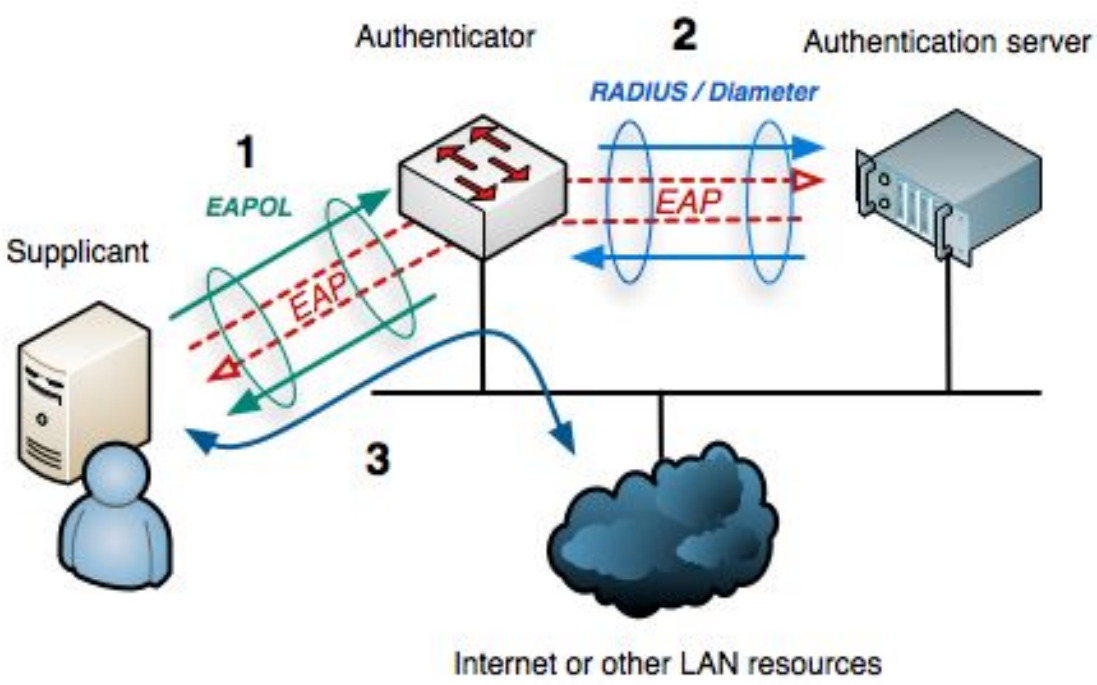
\includegraphics[scale=0.4]{../../immagini/eapol_scheme}
    \end{figure}\\\\
Il supplicant è un client 802.1X, all'inizio l'authenticator (switch) blocca tutto il traffico dal supplicant e lo manda solo verso l'auths server e quando questo si autentica comincia a forwardarne il traffico.

\subsection{EAP}
EAP è un framework di autenticazione, non implementa di per se un protocollo di autenticazione, bensì solo come trasportare al suo interno un protocollo per l'autenticazione, quindi per l'interfaccia ed il formato.
\\Quindi se TLS vuole essere incapsulato in EAP, bisogna definire come deve avvenire questo incapsulamento.
\\Ci sono diversi metodi di autenticazione supportati, anche vendor specific
\begin{itemize}
    \item EAP-MD5;
    \item EAP-POTP;
    \item EAP-GTC;
    \item EAP-TLS;
    \item ...
\end{itemize}

\subsection{RADIUS}
RADIUS (Remote Authentication Dila-In User Service) è un altro protocollo dell'architettura 802.1X ed è la scelta standard per l'autenticazione in 802.1X.
\\È un protocollo client server che gira a livello applicativo, può usare sia TCP che UDP.
\\I server di accesso alla rete spesso hanno anche un client RADIUS che comunica con un server RADIUS (spesso si usa però DIAMETER).

\section{802.1X overview}
802.1X usa classicamente un sistema di autenticazione dell'utente di tipo client/server con 3 componenti:
    \begin{itemize}
        \item client o supplicant;
        \item Access Device, ovvero authenticator;
        \item Authentication server, tipicamente un server RADIUS o DIAMETER, che mantiene le informazioni per l'autenticazione
    \end{itemize}
Usando EAP, il supplicant mette i messaggi EAP in Ethernet, tra auth e server auth dipende dal protocollo usato.
\\EAP può girare senza IP, è comodo perché la prima cosa da fare quando si accede ad una rete è autenticarsi ed essere autorizzati all'accesso.
\\Ci sono due modalità di autenticazione:
    \begin{itemize}
        \item EAP termination mode: usiamo il classico protocollo RADIUS, quindi col metodo usato da RADIUS, il pacchetto EAP è incalsulato dentro quello RADIUS;
        \item EAP relay mode: l'access device prende lo stesso EAP preso dal client e lo mette nel pacchetto di RADIUS (EAP over RADIUS) e trasmette questi pacchetti in una rete complessa verso l'auth server.
    \end{itemize}

\subsection{EAPOL}
La complessità è relazionata al metodo di autenticazione usato, difatti EAPOL ha una struttura di pacchetto molto semplice:
    \begin{itemize}
        \item PAE Ethernet Type
        \item Protocol version
        \item Type: 4 possibili
        \begin{itemize}
            \item EAP-Packet
            \item EAPoL-Start
            \item EAPoL-Logoff
            \item EAPoL-Key: usato per scambiare materiale di chiavi
        \end{itemize}
        \item length
        \item packet body
    \end{itemize}

Se il type è EAP, abbiamo un pacchetto EAP, anche in questo caso il pacchetto è semplice:
    \begin{itemize}
        \item Code: 1 byte, 4 tipi di messaggi
        \begin{itemize}
            \item Request: il messaggio del client è incapsulato in un Request packet
            \item Response: messaggio di risposta mandato dall'authenticator
            \item Success
            \item Failure
        \end{itemize}
        \item ID: 1 byte, usato per fare il matching fra il pacchetto di Response ed il corrispettivo pacchetto di Request
        \item Length
        \item Data: se il tipo è request o response c'è payload 
    \end{itemize}

\subsection{EAPOR}
Incapsula i pacchetti in RADIUS, per supportare EAP relay.
\\RADIUS usa gli attributi, il tipo 79 supporta EAP, inoltre sono stati aggiunti degli attributi a RADIUS:
\begin{itemize}
    \item EAP-Message: usato per incapsulare i pacchetti EAP
    \item Message-Authenticator: usato per verifcare ad autenticare i pacchetti di autenticazione in modo da proteggersi da spoofing o pacchetti non validi
\end{itemize}

\section{Processo di autenticazione in EAP}
\subsection{EAP in relay mode}
Se usiamo una MD5 challange-auth mode in relay mode, questi sono i messaggi scambiati:\\
    \begin{figure}[h!]
        \centering
        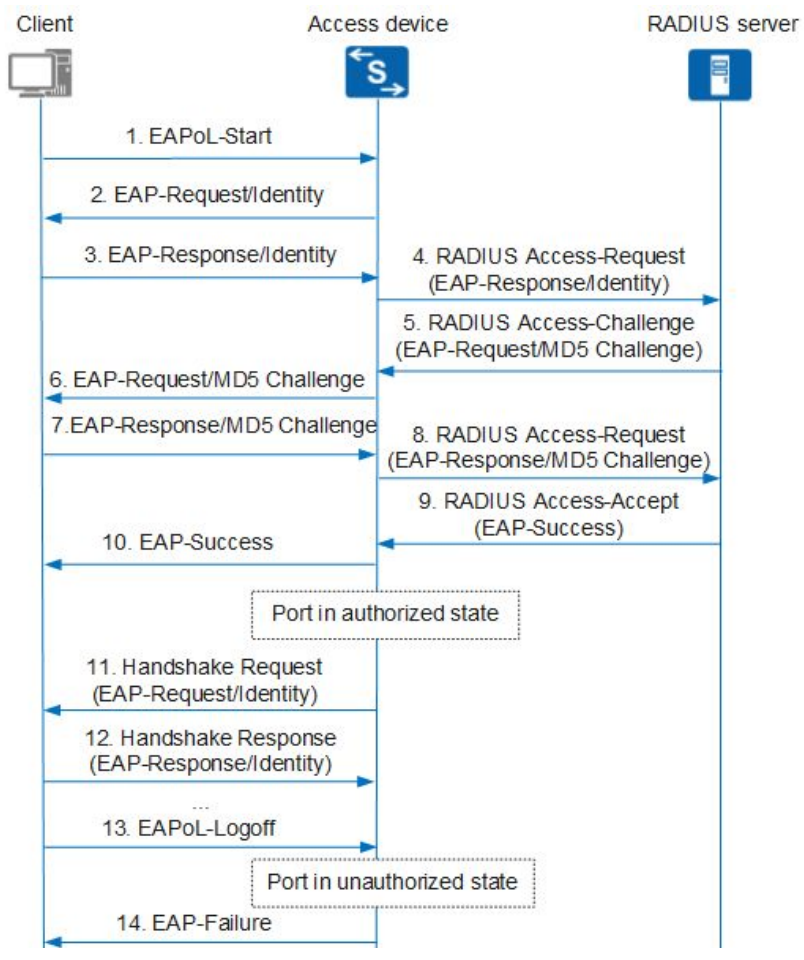
\includegraphics[scale=0.4]{../../immagini/eap_relay}
    \end{figure}
\\\\Come avviene lo scambio:
    \begin{itemize}
        \item parte tutto con lo start: l'utente registra username e password ed inizializza una richiesta di connessione.
        \\Viene quindi mandato il pacchetto EAPoL-Start
        \item l'access device restituisce l'EAP-Request/Identify per richiedere al cliente la sua identità
        \item il client risponde con un EAP-Response/Identity contente il suo user name per accedere al dispositivo
        \item l'access device incapsula il pacchetto di EAP-Response/Identity nel pacchetto di Access-Request RADIUS e lo manda al server di autenticazione
        \item dopo aver ricevuto il pacchetto, contente anche lo user name, il server cerca nel database una corrispondenza con la password, la cifra e genera una challenge MD5 casuale, mandando in risposta il RADIUS Access-Challenge 
        \item l'access device forwarda la challenge MD5 al client
        \item il client cifra la password e la challenge, genera un EAP-Response/MD5-Challenge e lo manda all'access device (Hash MD5 dell'ID del messaggio EAP + la stringa di challenge + la password utente)
        \item l'access device incapsula il pacchetto dell'utente in un pacchetto RADIUS Access-Request e lo manda al server
        \item il server confronta la password cifrata ricevuta con quella locale.
        \\Se c'è matching, l'utente è considerato valido dal server e quest'ultimo manda un RADIUS Access-Accept all'access device
        \item l'access device quindi manda un EAP-Success al client, cambiando lo stato della porta ad autorizzato e permettendo all'utente di accedere alla rete mediante questa porta
        \item quando l'utente è online, l'access device manda un pacchetto di \textbf{handshake} periodicamente per monitorare il client
        \item ricevuto tale pacchetto, il client manda come risposta un pacchetto che indica che è ancora online.
        \\Per default, l'access device disconnette l'utente se non riceve risposta entro 2 handshake consecutivi
        \item per andare offline, il client manda un EAPoL-Logoff 
    \end{itemize}
Periodicamente è possibile mandare dei messaggi di controllo per vedere se il client è ancora attivo:
    \begin{itemize}
        \item se il client va via, serve chiudere la porta o qualcun altro arriva e si autentica come il client
        \item può esserci accounting, quindi serve controllare se il client è attivo
    \end{itemize}

\subsection{EAP-TLS}
Lo scambio di messaggi è più complesso, ma il meccanismo è sempre lo stesso: si incapsulano dei messaggi di tipo TSL in un messaggio EAP, quindi nuovamente EAP trasporta solo i messaggi dei protocolli di autenticazione.

\subsection{Operazioni aggiuntive}
Fra le operazioni aggiunte, c'è la re-autenticazione utente:
    \begin{itemize}
        \item per utenti 802.1X autenticati: se l'amministratore modifica i parametri, come diritti di accesso o attributi di autorizzazione di un utente online o del server di autenticazione, l'utente deve ri-autenticarsi.
        \\L'access device manda i parametri di autenticazione al server per la ri-autenticazione.
        \\Se le informazioni del server rimangono invariate, l'utente rimane online, altrimenti viene disconnesso e deve ri-autenticarsi
        \item utente in stato di autenticazione anormale: l'access device salva le entry per utenti in stato di pre-connessione, ovvero che non si sono ancora autenticati o che hanno fallito l'autenticazione.
        \\Si può configurare il device di accesso per far si che questi utenti vengano ri-autenticati così da avere un accesso legittimo alla rete, ma se l'utente fallisce la ri-autenticazione prima che l'entry corrispondente scada, l'access device cancella l'entry e reclama i permessi di accesso alla rete concessi.
        \\Se invece un utente si ri-autentica con successo prima che la entry scada, l'access device aggiunge una entry di "user-authenticated" e fornisce i permessi di accesso alla rete.
    \end{itemize}
Quando l'utente va offline ma l'access device ed il server RADIUS non rilevano l'evento, possono incorrere problemi:
    \begin{itemize}
        \item il server RADIUS può continuare a fare accounting per l'utente
        \item utenti non autorizzati possono spoofare l'IP ad il MAC utente per ottenere accesso
        \item se ci sono molti utenti offline, potrebbero comunque essere contati come utenti che sono dentro, quindi altri utenti potrebbero non riuscire ad entrare.
    \end{itemize}
L'access device deve quindi rilevare il logout immediatamente, cancellare la entry utente e far si che il server fermi l'accounting.
\\802.1X si basa su diversi timer che controllano il numero di ritrasmissioni di pacchetti e di intervalli di timeout

\section{Autorizzazione in 802.1X}
\subsection{802.1X Authorization: VLAN}
È la per user membership della VLAN: se vogliamo assegnare la VLAN ad un utente specifico, abbiamo bisogno di poter autenticare l'utente ed in base all'identità dell'utente si decide di quale VLAN fa parte.
\\

\subsection{802.1X Authorization: ACL}
Possono esserci diverse ACL per diversi utenti, quindi è necessario incapsulare le ACL in EAP per poter determinare chi può fare cosa.
\\L'associazione delle ACL agli utenti sono nel RADIUS server, e possono essere assegnate:
    \begin{itemize}
        \item statiche: il server RADIUS usa gli attributi RADIUS standard di Filter-ID per assegnare un ACL ID all'utente.
        \\In questa modalità, l'ACL e la regola corrispondente sono configurate sull'access device
        \item dinamica: il server usa l'attributo HW-Data-Filter esteso da Huawei per assegnare un ACL ID e la corrispondente regola all'utente.
        \\Qui, ACL e regola sono configurate dal server stesso
    \end{itemize}

\subsection{802.1X Authorization: UCL}
Possiamo specificare una ACL per un dato gruppo di utenti, sempre tramite EAP.
\\Un UCL è una collezione di terminali di rete come PC e smartphone, l'amministratore può aggiungere utenti che hanno lo stesso requisito di accesso alla rete ad una UCL e configurare una policiy di accesso per l'intera UCL.
\\Il server RADIUS assegna l'UCL ad uno specifico utente in 3 modi:
    \begin{itemize}
        \item mediante l'attributo Filter-ID
        \item usando l'attributo HW-UCL-Group esteso da Huawei
        \item serve configurare l'UCL e la policy di accesso alla rete sull'access device prima, indipendentemente dalla modalità di autorizzazione dell'UCL usata
    \end{itemize}

\section*{Lab 5}
Recap: usiamo 802.1X per l'autenticazione nelle aree locali. L'idea è di avere un device di accesso che fa da autenticatore, ad esempio switch, abbiamo i device che vogliono connettersi allo switch e all'indizio possono solo mandare pacchetti di autenticazione. Il 3° attore è il server di autenticazione.\\ 802.1X definisce un modo per incapsulare i pacchetti di sicurezza nelle trame Ethernet.\\\\ Vediamo l'authorization port based e l'assegnazione di VLAN con 802.1X, configuriamo un lab usando md5 challange-response come metodo di autenticazione. Per installare radius (freeradius), basta usare il pakcet manager di ubuntu. Cumulus è stato configurato per essere usato come switch di layer 3: nel lab precedente c'era un router CISCO, qui facciamo la stessa cosa permettendo l'IP forwarding in Cumulus.\\ Per RADIUS dobbiamo configurare il client, ma di RADIUS e non il supplicant che richiede l'accesso alla rete
\end{document}
